\chapter{Numerical MRI} \label{sec:numerical-mri}
    %\todoitemthree{Maybe regenerate graphs with units.}
    \todoitemone{Recheck that graph references correspond correctly.}

    This chapter presents a method for numerical MRI (or synthetic MRI), where MRI signals are computed numerically for some underpinning flow field. Specifically, we will use either a manufactured simple flow field, or a simulated velocity field using the blood flow model introduced in \S\ref{sec:modelling:blood-flow}, to compute the evolution of the nuclear magnetisation of particles following this velocity field --- from which a single measurement of the MRI signal is taken at the so-called echo time. This approach provides a means of comparing our computational flow fields with in vivo placental flow data obtained from MRI scans.
    
    In \S\ref{sec:numerical-mri:preliminaries}, we will introduce some preliminaries on how MRI scanners make their measurements. Next, \S\ref{sec:numerical-mri:algorithm} will present an algorithm for computing the MRI signals, which involves tracking the displacement of many particles that accumulate so-called magnetic spin due to an applied magnetic field, and measuring these spins at the so-called echo time. \S\ref{sec:numerical-mri:manufactured} will give some simple examples of MRI behaviour on some simple test flow fields at the voxel-level, before \S\ref{sec:numerical-mri:placental} presents MRI signals computed from our placental flow simulations. \S\ref{sec:numerical-mri:fitting} will fit the data to an empirical model of MRI signal attenuation. \S\ref{sec:numerical-mri:comparison} ties the chapter together, presenting results comparing MRI behaviour on in vivo placental scans and numerical MRI data from computational flow fields. \S\ref{sec:numerical-mri:summary} concludes the chapter with a summary of the presented results.

    \section{MRI preliminaries} \label{sec:numerical-mri:preliminaries}
        We will ultimately compare in silico placental MRI data with in vivo placental MRI data, but first we present an overview of how MRI scanners make their measurements and how we can replicate this numerically. An important characteristic of motion-sensitising MRI is its lack of uniqueness in specifying the underlying velocity field. In fact, there are many velocity fields that may give the same MRI measurements. This phenomenon is discussed further in \S\ref{sec:numerical-mri:manufactured}. This non-uniqueness property clearly causes complications when inferring underlying velocity fields from in vivo MRI data; the approach of this chapter is a first step to interpreting MRI data as flows by instead numerically calculating MRI signals from computational flow fields, and then comparing these numerical MRI signals directly with in vivo MRI signal data. The remainder of this section gives a description of the details presented in Chapter 9 of \citeauthor{bernsteinHandbookMRIPulse2004} \cite{bernsteinHandbookMRIPulse2004} on motion-sensitising gradients.
    
        An MRI image domain is made up of many non-overlapping voxels covering the area of interest. Voxels are rectangular cuboids, within which MRI makes its measurements\footnote{For simplicity, this thesis only considers MRI measurements in 2D; we will continue to use the word `voxels', rather than `pixels', to describe the 2D squares used in this thesis nevertheless.}. Within each voxel, there are a number of hydrogen particles, each of which has a magnetic spin $\phi$ associated with it. These individual particles are themselves sometimes referred to as \textit{spins}. The nuclear magnetisation of individual particles can be written as $M = e^{-i\phi}$. It is the magnitude of the collective nuclear magnetisation within each voxel that MRI measures, often referred to as the signal and denoted by $S$.
    
        A magnetic gradient is applied over the entire domain, where in this particular setup the magnetic field varies linearly from one side of the domain to the other. The size of this gradient is usually denoted by $G$ or $g$. Magnetic gradients of a selection of strengths are applied through so-called \textit{pulse profiles}, where the choice of pulse profile significantly changes the resulting MRI images. Typically, these pulse profiles are applied in succession three times: once for each of the coordinate directions. There are two main choices that make up the resulting magnetic gradient pulse profile: waveform and pulse sequence. Waveforms describe the shape of lobes in the sequence\footnote{In this context, `lobes' refer to the form of the gradient pulse, not placental lobes.}, where each period of non-zero magnetic gradient strength is referred to as a `lobe'; these lobes may be, for example, sinusoidal or rectangular. Pulse sequences describe the ordering and timing of the application of lobes. Figure \ref{fig:bernstein_9.4} is reproduced from \cite{bernsteinHandbookMRIPulse2004} and shows 3 different waveforms for the same pulse sequence for a magnetic gradient $G$ in a single direction. We note that the first row in this figure shows a radio frequency (RF) pulse; RF pulses are used in combination with magnetic gradients here to initially align magnetic spins in the same direction in an effect called \textit{refocusing}, and also to aid in the collection of signals. The remainder of this chapter does not explicitly talk about RF signals, as they are not important for our application, but we acknowledge that they are important in real MRI scanners.

        \begin{figure}
            \centering
            \includegraphics[width=0.6\textwidth]{diagrams/other-paper-figures/Bernstein_9.4.png}
            \caption{Figure 9.4 from \cite{bernsteinHandbookMRIPulse2004}, showing 3 commonly used diffusion-gradient waveforms in gradient-echo pulse sequences, in combination with an RF sequence.}
            \label{fig:bernstein_9.4}
        \end{figure}
    
        We will focus on pulsed-gradient spin echo (PGSE) motion-sensitising gradients, with a rectangular waveform, which use magnetic gradients to detect motion of hydrogen particles in tissues. Following \citeauthor{nguyenFiniteElementsMethod2014} \cite{nguyenFiniteElementsMethod2014}, we start by introducing a time profile, which is given by
        \begin{equation}
            f(t) = 
            \begin{cases}
                1,  & t \in [t_1, t_1 + \delta], \\
                -1, & t \in [t_1 + \Delta, t_1 + \Delta + \delta], \\
                0,  & \text{otherwise}, 
            \end{cases}
            \label{eq:time-profile}
        \end{equation}
        where $t=0$ corresponds to the spins being reset to $\phi=0$, $t_1$ is the starting time of the first gradient pulse, and $\delta$ and $\Delta$ respectively describe the length of the lobes and length between the first lobe starting and the second lobe starting. Measurements of the signal are then taken at the chosen echo time $t_E > t_1 + \Delta + \delta$. The evolution of $G$ between $t=0$ and $t=t_E\,\unit{\milli\second}$ is referred to as a \textit{sequence}. For this application, we fix $t_1 = \qty{3.2}{\milli\second}$, $\delta = \qty{15.9}{\milli\second}$, $\Delta = \qty{30.9}{\milli\second}$, and $t_E = \qty{53}{\milli\second}$ \cite{dellschaftHaemodynamicsHumanPlacenta2020}. $f(t)$ is illustrated in Figure \ref{fig:mri-gradient-profile:1}. From this, we can construct our magnetic gradient as  
        \begin{equation}
            \vec{G}(t) := g \left[ f(t-T_x) \vec{\hat{x}} + f(t-T_y) \vec{\hat{y}} + f(t-T_z) \vec{\hat{z}} \right],
            \label{eq:g}
        \end{equation}
        where $g$ is constant and controls the amplitude of $\vec{G}$, $\vec{\hat{\cdot}}$ denotes the unit vectors in the coordinate directions, and $T_x, T_y, T_z$ denote the starting times of each sequence for the $x$-, $y$-, and $z$-directions, respectively. The sequences are applied sequentially, as illustrated in Figure \ref{fig:mri-gradient-profile:3}.
    
        \begin{figure}
            \centering
            \begin{subfigure}{0.45\textwidth}
                

\tikzset{every picture/.style={line width=0.75pt}} %set default line width to 0.75pt        

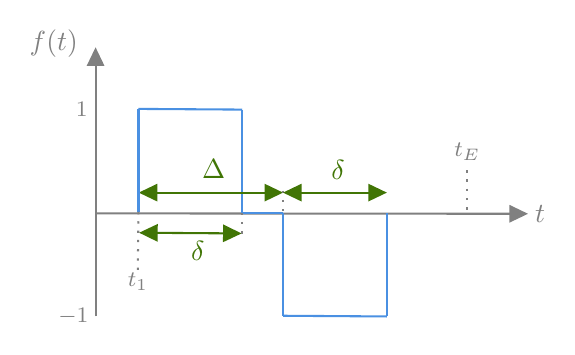
\begin{tikzpicture}[x=0.75pt,y=0.75pt,yscale=-1,xscale=1]
%uncomment if require: \path (0,300); %set diagram left start at 0, and has height of 300

%Straight Lines [id:da8882796881399757] 
\draw [color={rgb, 255:red, 128; green, 128; blue, 128 }  ,draw opacity=1 ]   (70.67,219.67) -- (70.67,93) ;
\draw [shift={(70.67,90)}, rotate = 90] [fill={rgb, 255:red, 128; green, 128; blue, 128 }  ,fill opacity=1 ][line width=0.08]  [draw opacity=0] (8.93,-4.29) -- (0,0) -- (8.93,4.29) -- cycle    ;
%Straight Lines [id:da664635011077519] 
\draw [color={rgb, 255:red, 128; green, 128; blue, 128 }  ,draw opacity=1 ]   (70.67,170) -- (276,170.2) ;
\draw [shift={(279,170.2)}, rotate = 180.06] [fill={rgb, 255:red, 128; green, 128; blue, 128 }  ,fill opacity=1 ][line width=0.08]  [draw opacity=0] (8.93,-4.29) -- (0,0) -- (8.93,4.29) -- cycle    ;
%Straight Lines [id:da17789798284277847] 
\draw [color={rgb, 255:red, 74; green, 144; blue, 226 }  ,draw opacity=1 ]   (91.33,119.67) -- (141.33,120) ;
%Straight Lines [id:da7626646796988461] 
\draw [color={rgb, 255:red, 74; green, 144; blue, 226 }  ,draw opacity=1 ]   (141.33,120) -- (141.33,169.67) ;
%Straight Lines [id:da4344394785262813] 
\draw [color={rgb, 255:red, 74; green, 144; blue, 226 }  ,draw opacity=1 ]   (141.33,169.67) -- (161,169.67) ;
%Straight Lines [id:da9282561195936812] 
\draw [color={rgb, 255:red, 74; green, 144; blue, 226 }  ,draw opacity=1 ]   (161,169.67) -- (161,219.33) ;
%Straight Lines [id:da08552867507313566] 
\draw [color={rgb, 255:red, 74; green, 144; blue, 226 }  ,draw opacity=1 ]   (161,219.33) -- (211,219.67) ;
%Straight Lines [id:da3575819731609853] 
\draw [color={rgb, 255:red, 74; green, 144; blue, 226 }  ,draw opacity=1 ]   (211,170) -- (211,219.67) ;
%Straight Lines [id:da12257132095246326] 
\draw [color={rgb, 255:red, 65; green, 117; blue, 5 }  ,draw opacity=1 ]   (94.67,179.35) -- (138,179.65) ;
\draw [shift={(141,179.67)}, rotate = 180.39] [fill={rgb, 255:red, 65; green, 117; blue, 5 }  ,fill opacity=1 ][line width=0.08]  [draw opacity=0] (8.93,-4.29) -- (0,0) -- (8.93,4.29) -- cycle    ;
\draw [shift={(91.67,179.33)}, rotate = 0.39] [fill={rgb, 255:red, 65; green, 117; blue, 5 }  ,fill opacity=1 ][line width=0.08]  [draw opacity=0] (8.93,-4.29) -- (0,0) -- (8.93,4.29) -- cycle    ;
%Straight Lines [id:da6443721529726347] 
\draw [color={rgb, 255:red, 65; green, 117; blue, 5 }  ,draw opacity=1 ]   (94.5,160) -- (158,160) ;
\draw [shift={(161,160)}, rotate = 180] [fill={rgb, 255:red, 65; green, 117; blue, 5 }  ,fill opacity=1 ][line width=0.08]  [draw opacity=0] (8.93,-4.29) -- (0,0) -- (8.93,4.29) -- cycle    ;
\draw [shift={(91.5,160)}, rotate = 0] [fill={rgb, 255:red, 65; green, 117; blue, 5 }  ,fill opacity=1 ][line width=0.08]  [draw opacity=0] (8.93,-4.29) -- (0,0) -- (8.93,4.29) -- cycle    ;
%Straight Lines [id:da43765182650583845] 
\draw [color={rgb, 255:red, 128; green, 128; blue, 128 }  ,draw opacity=1 ] [dash pattern={on 0.84pt off 2.51pt}]  (141.33,169.67) -- (141.33,180.33) ;
%Straight Lines [id:da9970970110276676] 
\draw [color={rgb, 255:red, 128; green, 128; blue, 128 }  ,draw opacity=1 ] [dash pattern={on 0.84pt off 2.51pt}]  (161,159) -- (161,169.67) ;
%Straight Lines [id:da9873905246267041] 
\draw [color={rgb, 255:red, 65; green, 117; blue, 5 }  ,draw opacity=1 ]   (164,160) -- (208,160) ;
\draw [shift={(211,160)}, rotate = 180] [fill={rgb, 255:red, 65; green, 117; blue, 5 }  ,fill opacity=1 ][line width=0.08]  [draw opacity=0] (8.93,-4.29) -- (0,0) -- (8.93,4.29) -- cycle    ;
\draw [shift={(161,160)}, rotate = 0] [fill={rgb, 255:red, 65; green, 117; blue, 5 }  ,fill opacity=1 ][line width=0.08]  [draw opacity=0] (8.93,-4.29) -- (0,0) -- (8.93,4.29) -- cycle    ;
%Straight Lines [id:da6590571773579443] 
\draw [color={rgb, 255:red, 128; green, 128; blue, 128 }  ,draw opacity=1 ] [dash pattern={on 0.84pt off 2.51pt}]  (249.73,149.2) -- (249.73,169.53) ;
%Straight Lines [id:da76362319772591] 
\draw [color={rgb, 255:red, 74; green, 144; blue, 226 }  ,draw opacity=1 ]   (91.33,119.67) -- (91.33,169.33) ;
%Straight Lines [id:da9036000522736403] 
\draw [color={rgb, 255:red, 128; green, 128; blue, 128 }  ,draw opacity=1 ] [dash pattern={on 0.84pt off 2.51pt}]  (91.33,169.33) -- (91,198.67) ;

% Text Node
\draw (63.6,88.2) node [anchor=east] [inner sep=0.75pt]  [color={rgb, 255:red, 128; green, 128; blue, 128 }  ,opacity=1 ]  {$f( t)$};
% Text Node
\draw (281,170.2) node [anchor=west] [inner sep=0.75pt]  [color={rgb, 255:red, 128; green, 128; blue, 128 }  ,opacity=1 ]  {$t$};
% Text Node
\draw (119.89,181.73) node [anchor=north] [inner sep=0.75pt]  [color={rgb, 255:red, 128; green, 128; blue, 128 }  ,opacity=1 ]  {$\textcolor[rgb]{0.25,0.46,0.02}{\delta }$};
% Text Node
\draw (127.55,142.4) node [anchor=north] [inner sep=0.75pt]  [color={rgb, 255:red, 128; green, 128; blue, 128 }  ,opacity=1 ]  {$\textcolor[rgb]{0.25,0.46,0.02}{\Delta }$};
% Text Node
\draw (187.55,154.99) node [anchor=south] [inner sep=0.75pt]  [color={rgb, 255:red, 128; green, 128; blue, 128 }  ,opacity=1 ]  {$\textcolor[rgb]{0.25,0.46,0.02}{\delta }$};
% Text Node
\draw (68.33,119.67) node [anchor=east] [inner sep=0.75pt]  [font=\footnotesize,color={rgb, 255:red, 128; green, 128; blue, 128 }  ,opacity=1 ]  {$1$};
% Text Node
\draw (68.67,219.67) node [anchor=east] [inner sep=0.75pt]  [font=\footnotesize,color={rgb, 255:red, 128; green, 128; blue, 128 }  ,opacity=1 ]  {$-1$};
% Text Node
\draw (91,197.4) node [anchor=north] [inner sep=0.75pt]  [font=\footnotesize,color={rgb, 255:red, 128; green, 128; blue, 128 }  ,opacity=1 ]  {$t_{1}$};
% Text Node
\draw (249.73,145.8) node [anchor=south] [inner sep=0.75pt]  [font=\footnotesize,color={rgb, 255:red, 128; green, 128; blue, 128 }  ,opacity=1 ]  {$t_{E}$};


\end{tikzpicture}

                \caption{}
                \label{fig:mri-gradient-profile:1}
            \end{subfigure}
            \hfill
            \begin{subfigure}{0.45\textwidth}
                

\tikzset{every picture/.style={line width=0.75pt}} %set default line width to 0.75pt        

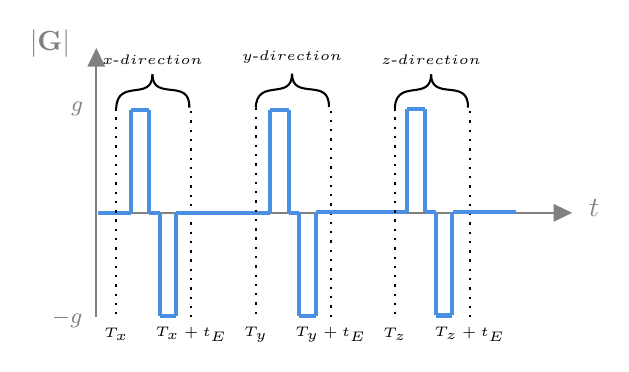
\begin{tikzpicture}[x=0.75pt,y=0.75pt,yscale=-1,xscale=1]
%uncomment if require: \path (0,300); %set diagram left start at 0, and has height of 300

%Straight Lines [id:da3774100901335702] 
\draw [color={rgb, 255:red, 128; green, 128; blue, 128 }  ,draw opacity=1 ]   (47.45,220) -- (47.45,93.33) ;
\draw [shift={(47.45,90.33)}, rotate = 90] [fill={rgb, 255:red, 128; green, 128; blue, 128 }  ,fill opacity=1 ][line width=0.08]  [draw opacity=0] (8.93,-4.29) -- (0,0) -- (8.93,4.29) -- cycle    ;
%Straight Lines [id:da9079908652045672] 
\draw [color={rgb, 255:red, 128; green, 128; blue, 128 }  ,draw opacity=1 ]   (48.07,169.75) -- (273.72,169.75) ;
\draw [shift={(276.72,169.75)}, rotate = 180] [fill={rgb, 255:red, 128; green, 128; blue, 128 }  ,fill opacity=1 ][line width=0.08]  [draw opacity=0] (8.93,-4.29) -- (0,0) -- (8.93,4.29) -- cycle    ;
%Straight Lines [id:da6473207409264472] 
\draw [color={rgb, 255:red, 74; green, 144; blue, 226 }  ,draw opacity=1 ][line width=1.5]    (64.04,120.08) -- (72.88,120.08) ;
%Straight Lines [id:da06919384086419744] 
\draw [color={rgb, 255:red, 74; green, 144; blue, 226 }  ,draw opacity=1 ][line width=1.5]    (72.88,120.08) -- (72.88,169.75) ;
%Straight Lines [id:da5657503776403818] 
\draw [color={rgb, 255:red, 74; green, 144; blue, 226 }  ,draw opacity=1 ][line width=1.5]    (72.88,169.75) -- (78.01,169.75) ;
%Straight Lines [id:da2035231243242186] 
\draw [color={rgb, 255:red, 74; green, 144; blue, 226 }  ,draw opacity=1 ][line width=1.5]    (78.01,169.75) -- (78.01,219.42) ;
%Straight Lines [id:da2770435671028688] 
\draw [color={rgb, 255:red, 74; green, 144; blue, 226 }  ,draw opacity=1 ][line width=1.5]    (78.01,219.42) -- (86,219.42) ;
%Straight Lines [id:da7146525103690513] 
\draw [color={rgb, 255:red, 74; green, 144; blue, 226 }  ,draw opacity=1 ][line width=1.5]    (86,169.75) -- (86,219.42) ;
%Straight Lines [id:da08072196166436374] 
\draw [color={rgb, 255:red, 74; green, 144; blue, 226 }  ,draw opacity=1 ][line width=1.5]    (64.04,120.08) -- (64.04,169.75) ;
%Straight Lines [id:da9026897276339403] 
\draw [color={rgb, 255:red, 74; green, 144; blue, 226 }  ,draw opacity=1 ][line width=1.5]    (48.07,169.75) -- (64.04,169.75) ;

%Straight Lines [id:da937386077900634] 
\draw  [dash pattern={on 0.84pt off 2.51pt}]  (93.13,120.75) -- (93.13,220.08) ;
%Curve Lines [id:da7511913583996024] 
\draw    (57.04,119.33) .. controls (57.61,104.67) and (74.5,116.33) .. (74.5,103) ;
%Curve Lines [id:da12325428458162424] 
\draw    (92.24,119) .. controls (92.8,104.33) and (74.5,116.33) .. (74.5,103) ;
%Straight Lines [id:da10398849489681083] 
\draw  [dash pattern={on 0.84pt off 2.51pt}]  (57.04,119.33) -- (57.04,220.25) ;
%Straight Lines [id:da08398923048196427] 
\draw [color={rgb, 255:red, 74; green, 144; blue, 226 }  ,draw opacity=1 ][line width=1.5]    (131.29,120.08) -- (140.13,120.08) ;
%Straight Lines [id:da32528202829910025] 
\draw [color={rgb, 255:red, 74; green, 144; blue, 226 }  ,draw opacity=1 ][line width=1.5]    (140.13,120.08) -- (140.13,169.75) ;
%Straight Lines [id:da8032661133457124] 
\draw [color={rgb, 255:red, 74; green, 144; blue, 226 }  ,draw opacity=1 ][line width=1.5]    (140.13,169.75) -- (145.26,169.75) ;
%Straight Lines [id:da3395149447265673] 
\draw [color={rgb, 255:red, 74; green, 144; blue, 226 }  ,draw opacity=1 ][line width=1.5]    (145.26,169.75) -- (145.26,219.42) ;
%Straight Lines [id:da6955133868719754] 
\draw [color={rgb, 255:red, 74; green, 144; blue, 226 }  ,draw opacity=1 ][line width=1.5]    (145.26,219.42) -- (153.25,219.42) ;
%Straight Lines [id:da011305796920654476] 
\draw [color={rgb, 255:red, 74; green, 144; blue, 226 }  ,draw opacity=1 ][line width=1.5]    (153.25,169.75) -- (153.25,219.42) ;
%Straight Lines [id:da4849350214011454] 
\draw [color={rgb, 255:red, 74; green, 144; blue, 226 }  ,draw opacity=1 ][line width=1.5]    (131.29,120.08) -- (131.29,169.75) ;
%Straight Lines [id:da5931104314922135] 
\draw [color={rgb, 255:red, 74; green, 144; blue, 226 }  ,draw opacity=1 ][line width=1.5]    (115.32,169.75) -- (131.29,169.75) ;

%Straight Lines [id:da8669231189933269] 
\draw  [dash pattern={on 0.84pt off 2.51pt}]  (160.38,120.5) -- (160.38,219.83) ;
%Curve Lines [id:da889044125391548] 
\draw    (124.29,119.08) .. controls (124.86,104.42) and (141.75,116.08) .. (141.75,102.75) ;
%Curve Lines [id:da9570400470225142] 
\draw    (159.49,118.75) .. controls (160.05,104.08) and (141.75,116.08) .. (141.75,102.75) ;
%Straight Lines [id:da32012167918494483] 
\draw  [dash pattern={on 0.84pt off 2.51pt}]  (124.29,119.08) -- (124.29,220) ;
%Straight Lines [id:da548151013698829] 
\draw [color={rgb, 255:red, 74; green, 144; blue, 226 }  ,draw opacity=1 ][line width=1.5]    (197.04,119.83) -- (205.88,119.83) ;
%Straight Lines [id:da7190010107515945] 
\draw [color={rgb, 255:red, 74; green, 144; blue, 226 }  ,draw opacity=1 ][line width=1.5]    (205.88,119.83) -- (205.88,169.5) ;
%Straight Lines [id:da5364622758177244] 
\draw [color={rgb, 255:red, 74; green, 144; blue, 226 }  ,draw opacity=1 ][line width=1.5]    (205.88,169.5) -- (211.01,169.5) ;
%Straight Lines [id:da22779131451799128] 
\draw [color={rgb, 255:red, 74; green, 144; blue, 226 }  ,draw opacity=1 ][line width=1.5]    (211.01,169.5) -- (211.01,219.17) ;
%Straight Lines [id:da946818978249186] 
\draw [color={rgb, 255:red, 74; green, 144; blue, 226 }  ,draw opacity=1 ][line width=1.5]    (211.01,219.17) -- (219,219.17) ;
%Straight Lines [id:da4540542047738241] 
\draw [color={rgb, 255:red, 74; green, 144; blue, 226 }  ,draw opacity=1 ][line width=1.5]    (219,169.5) -- (219,219.17) ;
%Straight Lines [id:da47688281363458307] 
\draw [color={rgb, 255:red, 74; green, 144; blue, 226 }  ,draw opacity=1 ][line width=1.5]    (197.04,119.83) -- (197.04,169.5) ;
%Straight Lines [id:da15791990154946056] 
\draw [color={rgb, 255:red, 74; green, 144; blue, 226 }  ,draw opacity=1 ][line width=1.5]    (181.07,169.5) -- (197.04,169.5) ;

%Straight Lines [id:da21285085567206097] 
\draw  [dash pattern={on 0.84pt off 2.51pt}]  (227.38,120.75) -- (227.38,220.08) ;
%Curve Lines [id:da4611087330179324] 
\draw    (191.29,119.33) .. controls (191.86,104.67) and (208.75,116.33) .. (208.75,103) ;
%Curve Lines [id:da5611948742808552] 
\draw    (226.49,119) .. controls (227.05,104.33) and (208.75,116.33) .. (208.75,103) ;
%Straight Lines [id:da7247349322588634] 
\draw  [dash pattern={on 0.84pt off 2.51pt}]  (191.29,119.33) -- (191.29,220.25) ;
%Straight Lines [id:da47838174999972116] 
\draw [color={rgb, 255:red, 74; green, 144; blue, 226 }  ,draw opacity=1 ][line width=1.5]    (86,169.75) -- (115.32,169.75) ;
%Straight Lines [id:da561199135094695] 
\draw [color={rgb, 255:red, 74; green, 144; blue, 226 }  ,draw opacity=1 ][line width=1.5]    (153.25,169.5) -- (183.25,169.5) ;
%Straight Lines [id:da23861894222113644] 
\draw [color={rgb, 255:red, 74; green, 144; blue, 226 }  ,draw opacity=1 ][line width=1.5]    (219.5,169.25) -- (249.75,169.25) ;

% Text Node
\draw (36.35,88.2) node [anchor=east] [inner sep=0.75pt]  [color={rgb, 255:red, 128; green, 128; blue, 128 }  ,opacity=1 ]  {$|\mathbf{G} |$};
% Text Node
\draw (283.36,167.53) node [anchor=west] [inner sep=0.75pt]  [color={rgb, 255:red, 128; green, 128; blue, 128 }  ,opacity=1 ]  {$t$};
% Text Node
\draw (42.54,119.67) node [anchor=east] [inner sep=0.75pt]  [font=\footnotesize,color={rgb, 255:red, 128; green, 128; blue, 128 }  ,opacity=1 ]  {$g$};
% Text Node
\draw (42.21,220.67) node [anchor=east] [inner sep=0.75pt]  [font=\footnotesize,color={rgb, 255:red, 128; green, 128; blue, 128 }  ,opacity=1 ]  {$-g$};
% Text Node
\draw (74.5,99.6) node [anchor=south] [inner sep=0.75pt]  [font=\tiny]  {$x\text{\mbox{-}direction}$};
% Text Node
\draw (57.04,223.65) node [anchor=north] [inner sep=0.75pt]  [font=\tiny]  {$T_{x}$};
% Text Node
\draw (93.13,223.48) node [anchor=north] [inner sep=0.75pt]  [font=\tiny]  {$T_{x} +t_{E}$};
% Text Node
\draw (141.75,99.35) node [anchor=south] [inner sep=0.75pt]  [font=\tiny]  {$y\text{\mbox{-}direction}$};
% Text Node
\draw (124.29,223.4) node [anchor=north] [inner sep=0.75pt]  [font=\tiny]  {$T_{y}$};
% Text Node
\draw (160.38,223.23) node [anchor=north] [inner sep=0.75pt]  [font=\tiny]  {$T_{y} +t_{E}$};
% Text Node
\draw (208.75,99.6) node [anchor=south] [inner sep=0.75pt]  [font=\tiny]  {$z\text{\mbox{-}direction}$};
% Text Node
\draw (191.29,223.65) node [anchor=north] [inner sep=0.75pt]  [font=\tiny]  {$T_{z}$};
% Text Node
\draw (227.38,223.48) node [anchor=north] [inner sep=0.75pt]  [font=\tiny]  {$T_{z} +t_{E}$};


\end{tikzpicture}

                \caption{}
                \label{fig:mri-gradient-profile:3}
            \end{subfigure}
            \caption{(a) Sketch of the time profile given in Equation \eqref{eq:time-profile} between $t=0$ and $t=t_E$. (b) Magnetic gradients applied sequentially in the 3 coordinate directions, for which the magnitude of the magnetic gradients is illustrated here. For each sequence, the spin is initialised $\phi = 0$ at $t = T_x, T_y, T_z$, and measurements are taken at $t = T_x + t_\text{E}$, $t = T_y + t_\text{E}$, and $t = T_z + t_\text{E}$.}
            \label{fig:mri-gradient-profile}
        \end{figure}
    
        The so-called $b$-value parameterises the magnetic gradient strength, related to $\vec{G}(t)$ through the following \cite{bernsteinHandbookMRIPulse2004}:
        \begin{equation}
            b = (2\gamma)^2 \int_0^{t_E} \norm{\vec{k}(t)}^2 \diff t,
        \end{equation}
        where $\vec{k}$ is defined by
        \begin{equation}
            \vec{k}(t) = \frac{\gamma^2}{2\pi} \int_0^t \vec{G}(s) \diff s,
        \end{equation}
        and $\gamma$ is the gyromagnetic ratio \cite{bernsteinHandbookMRIPulse2004}, fixed as $\gamma = 42.57 \times 2\pi \times 10^6$~\unit{\radian\per\second\per\tesla} for our application \cite{dellschaftHaemodynamicsHumanPlacenta2020}. Using Equations \eqref{eq:time-profile} and \eqref{eq:g}, \citeauthor{lebihanDiffusionPerfusionMagnetic1995} \cite{lebihanDiffusionPerfusionMagnetic1995} states that this relation may be simplified to
        \begin{equation}
            b = \gamma^2 g^2 \delta^2 (\Delta - \delta/3),
            \label{eq:g-to-b}
        \end{equation}
        where we assume that the sequences are non-overlapping (i.e., $T_x + t_E < T_y$ and $T_y + t_E < T_z$).
    
        An isochromat is an ensemble of individual particles on a scale smaller than voxels, whose individual magnetic spins $\phi$ are assumed to evolve in the same way \cite{jungSpinEchoMagnetic2013}. Depending upon the strength of the magnetic field at an isochromat's location, the magnetic spin may evolve differently. The evolution of the $j$th isochromat's spin is given by
        \begin{equation}
            \phi_j(t) = \gamma \int_0^t \vec{G}(\tau) \cdot \vec{r}_j(\tau) \diff \tau,
            \label{eq:phi}
        \end{equation}
        where $\vec{r}_j$ is the displacement of the $j$th isochromat, given as $\vec{r}_j(t) = \vec{x}_j(t) - \vec{x}_j(0)$, and $\vec{x}_j(t)$ is the position of the $j$th isochromat at time $t$ (see \cite{bernsteinHandbookMRIPulse2004}). We note here that this corresponds to integrating the Bloch-Torrey equation in Equation \eqref{eq:bloch-torrey} with $\vec{D} = \vec{0}$ (i.e., the Bloch equation \cite{bernsteinHandbookMRIPulse2004}); this simplification is made due to the stronger effects of so-called pseudo-diffusion present in studies of blood flow \cite{torreyBlochEquationsDiffusion1956,lebihanWhatCanWe2019}.
        
        The MRI signal itself is measured at the echo time, $t_E$. For a magnetic gradient applied only in one axis direction, the complex nuclear magnetisation at time $t$ for the $j$th isochromat is given by \cite{bernsteinHandbookMRIPulse2004} to be
        \begin{equation}
            M_j(t) := e^{-\iu\phi_j(t)}.
        \end{equation}
        The total nuclear magnetisation in a voxel at time $t$ is then given by 
        \begin{equation}
            \bar{M}(t) := \sum^{N_x}_{j=1} M_j(t),
            \label{eq:nuclear-magnetisation}
        \end{equation}
        and the corresponding signal at the echo time is given by
        \begin{equation}
            S_x := \left| \bar{M}(T_x + t_\text{E}) \right|,
            \label{eq:signal-x}
        \end{equation}
        where the sum is over all $N_x$ isochromats in a given voxel. Similar expressions follow for $S_y$ and $S_z$; for clarity, we have
        \begin{equation}
            S_y := \left| \bar{M}(T_y + t_\text{E}) \right|,
        \end{equation}
        \begin{equation}
            S_z := \left| \bar{M}(T_z + t_\text{E}) \right|.
        \end{equation}
        The total signal in a given voxel is then computed as 
        \begin{equation}
            S := S_x + S_y + S_z.
            \label{eq:total-s}
        \end{equation}

        Our approach here focusses on motion-sensitising MRI, where the dependence of $S$ upon $b$ can help reveal flow characteristics. We will now introduce an algorithm for computing $S$ for a given $b$, where particles are advected by an underlying velocity field.

    \section{Algorithm for computing numerical MRI signals} \label{sec:numerical-mri:algorithm}
        For all the simulations presented throughout the remainder of Chapter \ref{sec:numerical-mri}, we take voxels of size \qtyproduct{2.5x2.5}{\milli\metre} spanning the entire domain of interest. We then distribute the initial positions of many isochromats such that there are $20 \times 20$ equally-spaced isochromats in each voxel, where the $j$th isochromat's initial position is denoted by $\vec{x}^0_j$. Given the initial positions of each isochromat, we evolve the position of each isochromat according to the following:
        \begin{equation}
            \vec{x}^{n+1}_j = \vec{x}^n_j + \vec{u}(\vec{x}^0_j) ~ \Delta t,
        \end{equation}
        for time points $t^n$ between $t=0$ and $t=t_E$: $\{ t^n := n \Delta t \mid 0 \leq n \leq N_t \}$. Note that we fix $\vec{u}$ at $t = 0$ for computational simplicity. We discretise spin evolution from Equation \eqref{eq:phi} in a similar way:
        \begin{equation}
            \phi^{n+1}_j = \phi^n_j + \gamma \, \vec{G}(T_d + t^{n+1}) \cdot (\vec{x}^{n+1}_j - \vec{x}^0_j) ~ \Delta t,
        \end{equation}
        where $T_d$ is replaced by one of $T_x, T_y, T_z$ depending upon the coordinate direction in which the spins are being measured.
        
        Algorithm \ref{alg:mri} gives the general algorithm for computing $S$, which is calculated over every voxel and many choices of $b$. In specific terms for our application, we start by selecting the set of isochromat positions that lie in the given voxel. We next obtain a steady-state velocity field; \S\ref{sec:numerical-mri:manufactured} will use some simple manufactured flow fields, whereas \S\ref{sec:numerical-mri:placental} will use a placental velocity field obtained from Chapters \ref{sec:modelling} and \ref{sec:numerical-methods}. For each $b$, we calculate $\vec{G}(t)$ given in Equation \eqref{eq:g}, where $g$ is calculated through Equation \eqref{eq:g-to-b}, and $b$ is chosen as $5001$ equally-spaced values between $b=\qty{0}{\second\per\milli\metre^2}$ and $b=\qty{500}{\second\per\milli\metre^2}$. For simplicity, we take $531$ equally-spaced time points between $t=0$ and $t = t_E \equiv \qty{53}{\milli\second}$. In each voxel, a value of $S$ is computed for every value of $b$; calculations for each $S$ can therefore be done independently, which allows for easy parallel execution if desired. We note that this procedure may advect isochromats outside the voxel in which they are being measured; this isn't significant due to the short timescales and slow velocities involved. 
        
        \begin{algorithm}
            \SetKwInOut{Input}{input}
            \SetKwInOut{Output}{output}
            \Input{$\{\bar{\vec{x}}_j\}$: Set of sampled initial positions for each of the $N_x$ isochromats. \\
                   $\vec{u}(\vec{x})$: Steady velocity field. \\
                   $\vec{G}(t)$: Gradient sequence for a particular field strength, $b$. \\
                   $\{t^n\}$: Set of $N_t$ time-steps, each separated by $\Delta t$. \\
            }
            \ForEach{$d \in \{ \mlq x \mrq, \mlq y \mrq, \mlq z \mrq \}$ (dimension)}{
                Initialise spins for all isochromats: $\{ \phi_j^0 \} \gets \{0\}$ \\
                Initialise positions for all isochromats: $\{ \vec{x}_j^0 \} \gets \{\bar{\vec{x}}_j\}$ \\
                \For{$n = 0$ \KwTo $N_t - 1$ (time-steps)}{
                    \For{$j = 1$ \KwTo $N_x$ (isochromats)}{
                        $\vec{x}_j^{n+1} \gets \vec{x}_j^n + \vec{u}(\vec{x}_j^0) ~ \Delta t$ \\
                        $\phi_j^{n+1} \gets \phi_j^n + \gamma ~ \vec{G}(T_d + t^{n+1}) \cdot (\vec{x}_j^{n+1} - \vec{x}_j^0) ~ \Delta t$
                    } 
                } 
                $S_d \gets \left| \sum_{j=1}^{N_x} \exp \left( -\iu \phi_j^{N_t} \right) \right|$
            } 
            $S \gets S_x + S_y + S_z$ \\
            \Output{$S$}
            \caption{Numerically generates a signal $S$, given: a set of initial positions for each isochromat, a steady-state velocity field, a gradient sequence, and a set of discretised time points. This algorithm is used in each voxel for every choice of $b$.}
            \label{alg:mri}
        \end{algorithm}

        We will now use some simple manufactured flows to understand the dependence of MRI signal ($S$) upon magnetic field strength ($b$) through $S$-vs-$b$ graphs. Graphs such as these are useful to study, as different patterns can provide insight into the underlying sub-voxel flow field.

    \section{MRI for simple manufactured flows} \label{sec:numerical-mri:manufactured}
        Here, we will present a series of carefully designed example cases aimed at understanding the behaviour of MRI signals over different 2D velocity fields. For simplicity, each example is defined on the domain $\Omega := [0, 1]^2 \unit{\metre^2}$, with a single voxel spanning the entire domain. We choose $5001$ equally-spaced $b$-values ranging \qtyrange{0}{500}{\second\per\milli\meter^2}, with a $20\times20$ grid of isochromats that are initially equally-spaced over $\Omega$. Some of these examples will then be referred to when discussing the results of \S\ref{sec:numerical-mri:placental}.

        \subsection{Shear flow} \label{sec:numerical-mri:manufactured:shear}
            In the following three examples, we have a velocity field describing shear flow, given by
            \begin{equation}
                \vec{u}(\vec{x}) =
                \begin{cases}
                    U_1 ~ \vec{\hat{y}} & \text{if } x < 0.5, \\
                    U_2 ~ \vec{\hat{y}} & \text{if } x \geq 0.5,
                \end{cases}
            \end{equation}
            where $U_1$ and $U_2$ are scaling constants, and $\vec{\hat{y}}$ is the unit normal vector in the $y$-direction. The following subsubsections consider three different choices of $U_1$ and $U_2$ and the effect these have on $S$.

            \subsubsection{Example 1} \label{sec:numerical-mri:manufactured:shear:1}
                We initially select $U_1 = \qty{0.005}{\metre\per\second}$ and $U_2 = \qty{0.01}{\metre\per\second}$. This velocity field is visualised in Figure \ref{fig:mri-shear-1:quiver}.

                We denote $S$, $S_x$, and $S_y$ at $b=0$ respectively by $S_0$, $S_{x,0}$, and $S_{y,0}$, and denote the normalised signals by
                \begin{subequations}
                    \begin{align}
                        \bar{S} & := S/S_0, \\
                        \bar{S}_x & := S_x/S_{x,0}, \\
                        \bar{S}_y & := S_y/S_{y,0}.
                    \end{align}
                \end{subequations}
                We note that $S = S_x + S_y$ here, since there is no $z$-component to the signal in the 2D simulations presented in this thesis; we also note that $\bar{S}, \bar{S}_x, \bar{S}_y \in [0, 1]$. Figure \ref{fig:mri-shear-1:s-vs-b} presents these normalised signals against $b$, where we see that $\bar{S}$ oscillates between $0.5$ and $1$, with a decreasing frequency as $b$ increases.

                To understand why the oscillations are confined between $0.5$ and $1$, let's consider Equation \eqref{eq:total-s}, which states that the total signal $S$ for this 2D example is composed of signals from both the $x$- and $y$-directions (for simplicity, we set $S_z \equiv 0$ for the 2D flows in this thesis). The blue and green lines in Figure \ref{fig:mri-shear-1:s-vs-b} respectively show the $x$- and $y$-components of the normalised signal ($\bar{S}_x$ and $\bar{S}_y$) plotted against $b$. In the case of this artificially-created 2D velocity field, there is no movement in the $x$-direction, and therefore isochromats experience no variation in magnetic field strength, consequently giving no signal loss for $S_x$ (i.e, $S_x \equiv 1$). We note that full signal will always be retained at $b=0$ ($\bar{S}_{x,0} = 1$ and $\bar{S}_{y,0} = 1$), and in the most extreme case $\bar{S}_y$ will lose all signal ($\bar{S}_y = 0$) for some $b > 0$. This therefore gives $\bar{S} = 1$ when $\bar{S}_y = 1$, and $\bar{S} = 0.5$ when $\bar{S}_y = 0$.
                
                To understand the frequency decrease, we recall Equation \eqref{eq:phi}, which shows that $\phi$ depends upon the integral of $\vec{G}$; in turn, Equation \eqref{eq:g-to-b} indicates that $b$ depends quadratically on $g$, meaning that the frequency decrease is quadratic in $b$. Figure \ref{fig:mri-shear-1:s-vs-g} instead plots $S$ against $g$, for which we see that the frequency is constant for increasing $g$.
                
                Figure \ref{fig:mri-shear-1:s-vs-b} shows that $\bar{S}_y$ oscillates between $0$ and $1$, and at minima the derivative is discontinuous. This effect where signal is recovered quickly from $S=0$ is sometimes known as a \textit{rebound} or \textit{rebounding}. The non-unity values of $\bar{S}_y$ can be explained by visualising the nuclear magnetisation using Equation \eqref{eq:nuclear-magnetisation}. Figure \ref{fig:mri-shear-1:b} shows the different values of $\bar{M}(T_y + t_E)$ for different choices of $b$, where the colour of the arrow varies from lightest green ($b=\qty{0}{\second\per\milli\metre^2}$) to darkest green ($b=\qty{2}{\second\per\milli\metre^2}$); we choose to only visualise $\bar{M}(T_y + t_E)$ here because there is no signal loss for $\bar{M}(T_x + t_E)$; this shows how $S_y$ decreases with increasing $b$ in this range. Although not illustrated, at approximately $b=\qty{10.5}{\second\per\milli\metre^2}$, the magnitude of $\bar{M}(T_y + t_E)$ (i.e., $S_y$) is approximately zero, giving a minimum in Figure \ref{fig:mri-shear-1:s-vs-b}, for which the derivative is discontinuous as $\bar{M}(T_y + t_E)$ passes through the origin.
                
                We recall from Equation \eqref{eq:nuclear-magnetisation} that $\bar{M}(T_y + t_E)$ is computed from the sum of several unit magnitude complex numbers which encode the spins for each individual isochromat; Figure \ref{fig:mri-shear-1:spins} visualises the set of all isochromats in the voxel for $b=\qty{2}{\second\per\milli\metre^2}$ denoted by $\{ M_j(T_y + t_E) \}$, with $\bar{M}(T_y + t_E)$ also shown. We highlight that the most important feature of this test case is that the isochromats are clustered into two groups, corresponding to the two choices of fluid speed on either side of the domain; this is due to Equation \eqref{eq:phi} and the dependence of spin $\phi$ upon the displacement $\vec{r}$, which will accumulate at one of two rates.

                \begin{figure}
                    \thisfloatpagestyle{empty}
                    %% SHEAR TEST (SPLIT)
                    %   Generated and plotted from test 1 in ./drivers/mri_tests.py.
                    %   Implicitly calls plot_quiver() in ./plotting/plot_mri_spins.py
                    \begin{subfigure}{0.5\textwidth}
                        \centering
                        \includegraphics[width=\textwidth]{diagrams/results-mri/simple-tests/mri-spins_quiver_2D_shear_test_1.png}
                        \caption{}
                        \label{fig:mri-shear-1:quiver}
                    \end{subfigure}
                    \\
                    \begin{subfigure}{0.4\textwidth}
                        \centering
                        \includegraphics[width=\textwidth]{diagrams/results-mri/simple-tests/mri-spins_sall-vs-b_2D_shear_test_1.png}
                        \caption{}
                        \label{fig:mri-shear-1:s-vs-b}
                    \end{subfigure}
                    \vspace{4mm} % Weird place, I know, but this is the only place that gave spacing between the 2nd and 3rd rows.
                    \begin{subfigure}{0.4\textwidth}
                        \centering
                        \includegraphics[width=\textwidth]{diagrams/results-mri/simple-tests/mri-spins_gall-vs-b_2D_shear_test_1.png}
                        \caption{}
                        \label{fig:mri-shear-1:s-vs-g}
                    \end{subfigure}
                    \begin{subfigure}{0.4\textwidth}
                        \centering
                        \includegraphics[width=\textwidth]{diagrams/results-mri/simple-tests/mri-spins_b_2D_shear_test_1.png}
                        \caption{}
                        \label{fig:mri-shear-1:b}
                    \end{subfigure}
                    \begin{subfigure}{0.4\textwidth}
                        \centering
                        \includegraphics[width=\textwidth]{diagrams/results-mri/simple-tests/mri-spins_avg_2D_shear_test_1.png}
                        \caption{}
                        \label{fig:mri-shear-1:spins}
                    \end{subfigure}
                    \caption{The shear flow example from \S\ref{sec:numerical-mri:manufactured:shear:1} with $U_1 = \qty{0.005}{\metre\per\second}$ and $U_2 = \qty{0.01}{\metre\per\second}$, showing visualisations of (a) the velocity field for each isochromat, (b) $S$ against $b$, (c) $S$ against $g$, (d) $\bar{M}(T_y + t_E)$ for different choices of $b$, and (e) individual isochromat values of $\{ M_j(T_y + t_E) \}$ for $b=\qty{2}{\second\per\milli\metre^2}$.}
                    \label{fig:mri-shear-1}
                \end{figure}

            \subsubsection{Example 2} \label{sec:numerical-mri:manufactured:shear:2}
                We will now give another example of a shear flow velocity field, which is visualised in Figure \ref{fig:mri-shear-2:quiver}, this time with $U_1 = \qty{0.0025}{\metre\per\second}$ and $U_2 = \qty{-0.0025}{\metre\per\second}$. Figure \ref{fig:mri-shear-2:s-vs-b} shows the $S$-vs-$b$ graph for this example. Interestingly, this graph is identical to the one shown in Figure \ref{fig:mri-shear-1:s-vs-b}. Figure \ref{fig:mri-shear-2:b} shows the values of $\bar{M}(T_y + t_E)$ from $b=\qty{0}{\second\per\milli\metre^2}$ (lightest green) to $b=\qty{2}{\second\per\milli\metre^2}$ (darkest green), which shows that the argument of the complex number $\bar{M}(T_y + t_E)$ (i.e., $\phi$) is unchanging, whilst the magnitude of $\bar{M}(T_y + t_E)$ (i.e., $S$) does change --- and does so in precisely the same way as the previous example. Lastly, Figure \ref{fig:mri-shear-2:spins} shows each individual isochromat's spin for $b = \qty{2}{\second\per\milli\metre^2}$, which are again clustered into two groups that are separated by the same phase as the previous example.
                
                Crucially, this second test is an example of the non-uniqueness of MRI signals when measuring two different flow fields; the important message here is that is it the difference in \text{relative} speed between the groups that causes gives the behaviour in $S$: since the difference between the two velocity scalings are equal in both examples ($|U_2 - U_1| = \qty{0.005}{\metre\per\second}$), they exhibit exactly the same signal curve against $b$. This is shown succinctly by Equation \eqref{eq:phi}, which shows that the evolution of $\phi$ depends upon the displacement of the isochromats, each of which displace with velocity $\vec{u}(\vec{x}^0)$.

                \begin{figure}
                    %% SHEAR TEST (OPPOSING DIRECTIONS)
                    %   Generated and plotted from test 2 in ./drivers/mri_tests.py.
                    %   Implicitly calls plot_quiver() in ./plotting/plot_mri_spins.py
                    \begin{subfigure}{0.4\textwidth}
                        \centering
                        \includegraphics[width=\textwidth]{diagrams/results-mri/simple-tests/mri-spins_quiver_2D_shear_test_2.png}
                        \caption{}
                        \label{fig:mri-shear-2:quiver}
                    \end{subfigure}
                    \vspace{4mm} % Weird place, I know, but this is the only place that gave spacing between the 1st and 2nd rows.
                    \begin{subfigure}{0.4\textwidth}
                        \centering
                        \includegraphics[width=\textwidth]{diagrams/results-mri/simple-tests/mri-spins_sall-vs-b_2D_shear_test_2.png}
                        \caption{}
                        \label{fig:mri-shear-2:s-vs-b}
                    \end{subfigure}
                    \begin{subfigure}{0.4\textwidth}
                        \centering
                        \includegraphics[width=\textwidth]{diagrams/results-mri/simple-tests/mri-spins_b_2D_shear_test_2.png}
                        \caption{}
                        \label{fig:mri-shear-2:b}
                    \end{subfigure}
                    \begin{subfigure}{0.4\textwidth}
                        \centering
                        \includegraphics[width=\textwidth]{diagrams/results-mri/simple-tests/mri-spins_avg_2D_shear_test_2.png}
                        \caption{}
                        \label{fig:mri-shear-2:spins}
                    \end{subfigure}
                    \caption{The shear flow example from \S\ref{sec:numerical-mri:manufactured:shear:2} with $U_1 = \qty{0.0025}{\metre\per\second}$ and $U_2 = \qty{-0.0025}{\metre\per\second}$, showing visualisations of (a) the velocity field for each isochromat, (b) $S$ against $b$, (c) $\bar{M}(T_y + t_E)$ for different choices of $b$, and (d) individual isochromat values of $\{ M_j(T_y + t_E) \}$ for $b=\qty{2}{\second\per\milli\metre^2}$.}
                    \label{fig:mri-shear-2}
                \end{figure}

            \subsubsection{Example 3} \label{sec:numerical-mri:manufactured:shear:3}
                One final example of shear flow is to take $U_1 = \qty{0.01}{\metre\per\second}$ and $U_2 = \qty{0.01}{\metre\per\second}$, which we note gives a constant flow. This velocity field is visualised in Figure \ref{fig:mri-shear-3:quiver}. The $S$-vs-$b$ graph is shown in Figure \ref{fig:mri-shear-3:s-vs-b}, which attains full signal for all choices of $b$. Because $U_2 - U_1 = 0$ here, Figure \ref{fig:mri-shear-3:spins} shows that there is no signal loss for all $b$. Although Figure \ref{fig:mri-shear-3:b} shows the angle of $\bar{M}(T_y + t_E)$ changing for different $b$, all the isochromats remain in a single group, therefore giving $\bar{S}=1$.
    
                \begin{figure}
                    %% SHEAR TEST (UNIFORM)
                    %   Generated and plotted from test 3 in ./drivers/mri_tests.py.
                    %   Implicitly calls plot_quiver() in ./plotting/plot_mri_spins.py
                    \begin{subfigure}{0.4\textwidth}
                        \centering
                        \includegraphics[width=\textwidth]{diagrams/results-mri/simple-tests/mri-spins_quiver_2D_shear_test_3.png}
                        \caption{}
                        \label{fig:mri-shear-3:quiver}
                    \end{subfigure}
                    \vspace{4mm} % Weird place, I know, but this is the only place that gave spacing between the 1st and 2nd rows.
                    \begin{subfigure}{0.4\textwidth}
                        \centering
                        \includegraphics[width=\textwidth]{diagrams/results-mri/simple-tests/mri-spins_sall-vs-b_2D_shear_test_3.png}
                        \caption{}
                        \label{fig:mri-shear-3:s-vs-b}
                    \end{subfigure}
                    \begin{subfigure}{0.4\textwidth}
                        \centering
                        \includegraphics[width=\textwidth]{diagrams/results-mri/simple-tests/mri-spins_b_2D_shear_test_3.png}
                        \caption{}
                        \label{fig:mri-shear-3:b}
                    \end{subfigure}
                    \begin{subfigure}{0.4\textwidth}
                        \centering
                        \includegraphics[width=\textwidth]{diagrams/results-mri/simple-tests/mri-spins_avg_2D_shear_test_3.png}
                        \caption{}
                        \label{fig:mri-shear-3:spins}
                    \end{subfigure}
                    \caption{The shear flow example from \S\ref{sec:numerical-mri:manufactured:shear:3} with $U_1 = \qty{0.01}{\metre\per\second}$ and $U_2 = \qty{0.01}{\metre\per\second}$, showing a visualisation of (a) the velocity field for each isochromat, (b) $S$ against $b$, (c) $\bar{M}(T_y + t_E)$ for different choices of $b$, and (d) individual isochromat values of $\{ M_j(T_y + t_E) \}$ for $b=\qty{2}{\second\per\milli\metre^2}$.}
                    \label{fig:mri-shear-3}
                \end{figure}

        \subsection{Rotational flow} \label{sec:numerical-mri:manufactured:rotational}
            For the next example of velocity field, we introduce a rotational flow, given by
            \begin{equation}
                \vec{u}(x, y) = \begin{pmatrix}-U_1 y / L \\ U_2 x / L\end{pmatrix},
            \end{equation}
            where $L = \qty{1}{\metre}$ is the length of the domain.
            For simplicity, we select $U_1 = \qty{0.01}{\metre\per\second}$ and $U_2 = \qty{0.01}{\metre\per\second}$, which gives the velocity field illustrated in Figure \ref{fig:mri-rotational:quiver}.
            
            The $S$-vs-$b$ graph is shown in Figure \ref{fig:mri-rotational:s-vs-b}; similar to the previous examples, we observe oscillations with decreasing frequency as $b$ increases (or equivalently constant frequency as $g$ increases). Figure \ref{fig:mri-rotational:b} also shows a familiar pattern for each $b$ to those shown in the shear flow examples. Figure \ref{fig:mri-rotational:spins} plots the individual spins for each isochromat for $b=\qty{2}{\second\per\milli\metre^2}$, which, unlike the previous examples, cluster into $20$ values associated with the number of isochromats lying in the $y$-direction. $b=\qty{9.4}{\second\per\milli\metre^2}$ corresponds to the first local minimum of $\bar{S} \approx 0$ in Figure \ref{fig:mri-rotational:s-vs-b}, which is where the isochromats become equally-separated and therefore give a signal of $\bar{S}=0$. Figure \ref{fig:mri-rotational:spins_min} shows the individual spins distributed equally for $b=\qty{9.4}{\second\per\milli\metre^2}$.
            
            We note that the amplitude of the oscillations decreases as $b$ increases in Figure \ref{fig:mri-rotational:s-vs-b}. In previous examples, full signal ($\bar{S}=1$) was regained through an effect known as \textit{refocusing} --- where spins coincide at $b>0$. Refocusing does not happen to the same extent here due to the spins clustering into $20$ values (due to the number of sample points), rather than just $2$. For $b = \qty{19.3}{\second\per\milli\metre^2}$, Figure \ref{fig:mri-rotational:s-vs-b} shows a local maximum of $\bar{S} \approx 0.22$. Figure \ref{fig:mri-rotational:spins_max} plots the individual spins again for this choice of $b$, which shows $14$ different phases in which isochromats cluster into, with $6$ of those phases in the lower right showing two isochromats overlapping (indicated by the darker gray arrow opacity). The lowering amplitude of $\bar{S}$ is therefore due to a weakening refocussing effect, where fewer isochromats overlap with the same phase, resulting in a gradually smaller value of $\bar{S}$.

            \begin{figure}
                %% ROTATIONAL TEST
                %   Generated and plotted from test 4 in ./drivers/mri_tests.py.
                %   Implicitly calls plot_quiver() in ./plotting/plot_mri_spins.py
                \begin{subfigure}{0.4\textwidth}
                    \centering
                    \includegraphics[width=\textwidth]{diagrams/results-mri/simple-tests/mri-spins_quiver_2D_rotational_test_4.png}
                    \caption{}
                    \label{fig:mri-rotational:quiver}
                \end{subfigure}
                \vspace{4mm} % Weird place, I know, but this is the only place that gave spacing between the 1st and 2nd rows.
                \begin{subfigure}{0.4\textwidth}
                    \centering
                    \includegraphics[width=\textwidth]{diagrams/results-mri/simple-tests/mri-spins_sall-vs-b_2D_rotational_test_4.png}
                    \caption{}
                    \label{fig:mri-rotational:s-vs-b}
                \end{subfigure}
                \begin{subfigure}{0.4\textwidth}
                    \centering
                    \includegraphics[width=\textwidth]{diagrams/results-mri/simple-tests/mri-spins_b_2D_rotational_test_4.png}
                    \caption{}
                    \label{fig:mri-rotational:b}
                \end{subfigure}
                \begin{subfigure}{0.4\textwidth}
                    \centering
                    \includegraphics[width=\textwidth]{diagrams/results-mri/simple-tests/mri-spins_avg_2D_rotational_test_4.png}
                    \caption{}
                    \label{fig:mri-rotational:spins}
                \end{subfigure}
                \begin{subfigure}{0.4\textwidth}
                    \centering
                    \includegraphics[width=\textwidth]{diagrams/results-mri/simple-tests/mri-spins_avg_2D_rotational_test_4_b9.4.png}
                    \caption{}
                    \label{fig:mri-rotational:spins_min}
                \end{subfigure}
                \begin{subfigure}{0.4\textwidth}
                    \centering
                    \includegraphics[width=\textwidth]{diagrams/results-mri/simple-tests/mri-spins_avg_2D_rotational_test_4_b19.3.png}
                    \caption{}
                    \label{fig:mri-rotational:spins_max}
                \end{subfigure}
                \caption{The rotational flow example from \S\ref{sec:numerical-mri:manufactured:rotational} with $U_1 = \qty{0.01}{\metre\per\second}$ and $U_2 = \qty{0.01}{\metre\per\second}$, showing visualisations of (a) the velocity field for each isochromat, (b) $S$ against $b$, and (c) $\bar{M}(T_y + t_E)$ for different choices of $b$. (d), (e), and (f) respectively show individual isochromat values of $\{ M_j(T_y + t_E) \}$ for $b=\qty{2}{\second\per\milli\metre^2}$, $b=\qty{9.4}{\second\per\milli\metre^2}$, and $b=\qty{19.3}{\second\per\milli\metre^2}$.}
                \label{fig:mri-rotational}
            \end{figure}

            % \begin{figure}
            %     \begin{subfigure}[b]{0.3\textwidth}
            %         \centering
            %         \includegraphics[width=\textwidth]{diagrams/results-mri/simple-tests/2D_rotational_test_s-vs-b_1_4.png}
            %         \caption{}
            %         \label{fig:mri-rotational:s-vs-b}
            %     \end{subfigure}
            %     \hfill
            %     \begin{subfigure}[b]{0.3\textwidth}
            %         \centering
            %         \includegraphics[width=\textwidth]{diagrams/results-mri/simple-tests/mri-spins_b_2D_rotational_test_4.png}
            %         \caption{}
            %         \label{fig:mri-rotational:b}
            %     \end{subfigure}
            %     \hfill
            %     \begin{subfigure}[b]{0.3\textwidth}
            %         \centering
            %         \includegraphics[width=\textwidth]{diagrams/results-mri/simple-tests/mri-spins_avg_2D_rotational_test_4.png}
            %         \caption{}
            %         \label{fig:mri-rotational:spins}
            %     \end{subfigure}
            %     \begin{subfigure}[b]{0.3\textwidth}
            %         \centering
            %         \includegraphics[width=\textwidth]{diagrams/results-mri/simple-tests/2D_accelerating_test_sx-vs-b_1_5}
            %         \caption{}
            %         \label{fig:mri-accelerating:s-vs-b}
            %     \end{subfigure}
            %     \hfill
            %     \begin{subfigure}[b]{0.3\textwidth}
            %         \centering
            %         \includegraphics[width=\textwidth]{diagrams/results-mri/simple-tests/mri-spins_b_2D_accelerating_test_5.png}
            %         \caption{}
            %         \label{fig:mri-accelerating:b}
            %     \end{subfigure}
            %     \hfill
            %     \begin{subfigure}[b]{0.3\textwidth}
            %         \centering
            %         \includegraphics[width=\textwidth]{diagrams/results-mri/simple-tests/mri-spins_avg_2D_accelerating_test_5.png}
            %         \caption{}
            %         \label{fig:mri-accelerating:spins}
            %     \end{subfigure}
            %     \caption{A rotational flow example from \S\ref{sec:numerical-mri:manufactured} with $U_1 = \qty{0.01}{\metre\per\second}$ and $U_2 = \qty{0.01}{\metre\per\second}$ with graphs in (a)--(c), and an accelerating flow example from \S\ref{sec:numerical-mri:manufactured} with $U = \qty{0.01}{\metre\per\second}$ and $X = \ln(10)$ with graphs in (d)--(f). (a) and (d) show $S$ or $S_x$ against $b$, (b) and (e) show $\bar{M}(T_y + t_E)$ for different choices of $b$, and (c) and (f) show individual isochromat values of $\{ M_j(T_y + t_E) \}$.}
            %     \label{fig:mri-rotational-and-accelerating}
            % \end{figure}

        \subsection{Accelerating flow} \label{sec:numerical-mri:manufactured:accelerating}
            In this final simple flow example, we have a velocity profile describing accelerating flow, given by
            \begin{equation}
                \vec{u}(\vec{x}) = U e^{X(x-L)} \hat{\vec{x}},
                \label{eq:mri-accelerating}
            \end{equation}
            where $U$ is a scaling for the velocity, $X$ is a scaling for the position, $L$ is the length of the domain, and $\vec{x} \equiv (x, y)^\intercal$. For simplicity, we select $U = \qty{-0.01}{\metre\per\second}$, $X = \qty{2.3026}{\per\metre}$, and $L = \qty{1}{\metre}$; we note that this choice of parameters yields a negatively accelerating flow (i.e., a decelerating flow) and is compressible (i.e., $\vec{\nabla} \cdot \vec{u} \neq 0$). Figure \ref{fig:mri-accelerating:quiver} visualises this velocity field.
            
            Figure \ref{fig:mri-accelerating:s-vs-b} shows the corresponding $S$-vs-$b$ graph, where we note that $\bar{S}_y \equiv 1$ because there is no flow in the $y$-direction, which is unlike the previous flow examples. We notice that $\bar{S}_x$ has oscillations, but none of these dephase enough to give $\bar{S}_x=0$, unlike the previous examples we have considered. Interestingly, the amplitude of the oscillations increases for increasing $b$, although the general trend of $\bar{S}_x$ decreases in value.
            
            Figure \ref{fig:mri-accelerating:b} shows $\bar{M}(T_x + t_E)$ between $b=\qty{0}{\second\per\milli\metre^2}$ (lightest blue) and $b=\qty{2}{\second\per\milli\metre^2}$ (darkest blue). In this chosen range of $b$, $\bar{M}(T_x + t_E)$ is quite similar to $\bar{M}(T_y + t_E)$ for the rotational flow presented in Figure \ref{fig:mri-rotational:spins}. However, as Figure \ref{fig:mri-accelerating:s-vs-b} shows, the values of $\bar{S}_x$ for higher $b$ are quite different due to $\bar{M}(T_x + t_E)$ not passing through the origin. Figure \ref{fig:mri-accelerating:spins} shows the individual spins of each isochromat, which, unlike the previous examples, are not evenly spaced around $\bar{M}(T_x + t_E)$; instead, there are a higher density of isochromat spins $\phi$ closer to zero. Carefully considering the rotational example in only the $y$-direction, we note that the isochromats have a linear variation in the velocity field, which leads to an equal distribution of spin accumulation rates; however, the accelerating flow instead has an exponential variation in the velocity field, which produces a higher density of slower-moving isochromats near $x=\qty{0}{\metre}$ (that displace a smaller amount than faster-moving isochromats near $x=\qty{1}{\metre}$), which in turn makes these isochromats accumulate less spin (see Equation \eqref{eq:phi}).

            \begin{figure}
                %% ACCELERATING TEST
                %   Generated and plotted from test 5 in ./drivers/mri_tests.py.
                %   Implicitly calls plot_quiver() in ./plotting/plot_mri_spins.py
                \begin{subfigure}{0.4\textwidth}
                    \centering
                    \includegraphics[width=\textwidth]{diagrams/results-mri/simple-tests/mri-spins_quiver_2D_accelerating_test_5.png}
                    \caption{}
                    \label{fig:mri-accelerating:quiver}
                \end{subfigure}
                \vspace{4mm} % Weird place, I know, but this is the only place that gave spacing between the 1st and 2nd rows.
                \begin{subfigure}{0.4\textwidth}
                    \centering
                    \includegraphics[width=\textwidth]{diagrams/results-mri/simple-tests/mri-spins_sall-vs-b_2D_accelerating_test_5.png}
                    \caption{}
                    \label{fig:mri-accelerating:s-vs-b}
                \end{subfigure}
                \begin{subfigure}{0.4\textwidth}
                    \centering
                    \includegraphics[width=\textwidth]{diagrams/results-mri/simple-tests/mri-spins_b_2D_accelerating_test_5.png}
                    \caption{}
                    \label{fig:mri-accelerating:b}
                \end{subfigure}
                \begin{subfigure}{0.4\textwidth}
                    \centering
                    \includegraphics[width=\textwidth]{diagrams/results-mri/simple-tests/mri-spins_avg_2D_accelerating_test_5.png}
                    \caption{}
                    \label{fig:mri-accelerating:spins}
                \end{subfigure}
                \caption{The accelerating flow example from \S\ref{sec:numerical-mri:manufactured:accelerating} with $U = \qty{-0.01}{\metre\per\second}$ and $X = \ln(10)$, showing (a) a visualisation of the velocity field for each isochromat, (b) $S$ against $b$, (c) $\bar{M}(T_x + t_E)$ for different choices of $b$, and (d) individual isochromat values of $\{ M_j(T_x + t_E) \}$ for $b=\qty{2}{\second\per\milli\metre^2}$.}
                \label{fig:mri-accelerating}
            \end{figure}

        \subsection{Summary of simple manufactured flows}
            These simple examples have given us an understanding of how local flow fields affect MRI signal, $S$, according to variations in the magnetic field strength, $b$. We inspected, in detail, the behaviour of individual isochromats under different velocity fields and their dependence upon the underlying velocity field, and what overall effect this has on a voxel's measured MRI signal.
            
            We found that almost all of our flow examples gave some sort of oscillatory behaviour in $S$ for increasing $b$, with the notable exception being constant flow, where maximum signal is always retained. In particular, we found several oscillating signals that recovered sharply from $S=0$, which are known as rebounds. We also found that the frequency of the aforementioned oscillations in $S$ decreased quadratically in $b$, due to the relationship between $b$ and $\vec{G}$.

            We also gave an example of two different shearing flow velocity fields that produced exactly the same MRI signals, thus demonstrating non-uniqueness in $S$-vs-$b$ patterns in specifying the underlying velocity field. The rotational flow example gave an amplitude reduction in the $S$ oscillations, which was due to a weakening refocussing effect; this was where only some of the individual isochromat phases coincided at local maxima, and therefore gave a lower overall signal. The accelerating flow example gave an interesting $S$-vs-$b$ graph, where the signal overall reduced, but actually increased in amplitude for $b > 50$. From this point onward, we will use $S$ in place of $\bar{S}$ to simplify the notation when it is clear that $S$ is normalised.

            We will now calculate MRI signals on a flow field computed from our model of placental blood flow.

    \section{MRI for placental flows} \label{sec:numerical-mri:placental}
        This section will briefly provide visualisations of real and simulated MRI data, which will be explored in greater depth in \S\ref{sec:numerical-mri:comparison}.
    
        The `standard' MRI pictures that are usually used in a medical setting are a 3D stack of 2D images in $x$-$y$ space showing $S$ in each voxel for a fixed $b$ (i.e., for a fixed choice of magnetic field strength). An example MRI image for $b=\qty{1}{\second\per\milli\metre^2}$ on a single $z$-slice of a \textit{real} placenta and surrounding area is shown in Figure \ref{fig:mri-real:S}. These pictures are often referred to as `signal maps'. Signal maps allow for study of changing $S$-value over a 3D stack of 2D $x$-$y$ slices, whereas the $S$-vs-$b$ graphs allow for study of changing $S$-value over different magnetic field strengths $b$. Although we will not explore signal maps in any great depth, we introduce them here to visualise placental structure for later discussion. Figure \ref{fig:mri-real:S-zoom} shows a zoomed-in view of Figure \ref{fig:mri-real:S}, with two voxels marked in blue and green for later discussion. 

        \begin{figure}
            %% REAL MRI DATA
            %   Generated and plotted from figures 1 and 2 in ./mri_code/plot_example_mri.m.
            \begin{centering}
                \begin{subfigure}{0.4\textwidth}
                    \begin{centering}
                        \includegraphics[width=\textwidth]{diagrams/results-mri/real-placenta/example-placenta-mri.png}
                        \caption{}
                        \label{fig:mri-real:S}
                    \end{centering}
                \end{subfigure}
                \begin{subfigure}{0.5\textwidth}
                    \begin{centering}
                        \includegraphics[width=\textwidth]{diagrams/results-mri/real-placenta/example-placenta-mri_zoomed.png}
                        \caption{}
                        \label{fig:mri-real:S-zoom}
                    \end{centering}
                \end{subfigure}
            \end{centering}
            \caption{(a) $S$ for $b=\qty{1}{\second\per\milli\metre^2}$ on a real MRI scan, showing the placenta and attached fetus, with (b) showing a zoomed in view on the red box. Two highlighted voxels are coloured in blue and green for later discussion. Data provided via private correspondence with George Hutchinson\protect\footnote{\href{mailto:george.hutchinson1@nottingham.ac.uk}{george.hutchinson1@nottingham.ac.uk}} and Penny Gowland\protect\footnote{\href{mailto:penny.gowland@nottingham.ac.uk}{penny.gowland@nottingham.ac.uk}}.}
            \label{fig:mri-real}
        \end{figure}

        We will now use the mathematical model of the blood flow field from Chapter \ref{sec:modelling}, with the numerical methods from Chapter \ref{sec:numerical-methods} to simulate blood flow in the placenta, and then use the algorithm from \S\ref{sec:numerical-mri:algorithm} to compute $S$ in each voxel for many choices of $b$. We will specifically choose the problem setup from \S\ref{sec:numerical-methods:blood-flow-experiments:asymmetric}, where basal plate veins have been placed asymmetrically. The flow field from this simulation is shown in Figure \ref{fig:asymmetric-placenta}, which is repeated here for convenience.

        \begin{figure}
            \begin{centering}
                % OVERALL FLOW
                %  Resulting from running ./drivers/mri_run.py
                %  Plotted in a separate plotter script ./plotting/placenta-plots.pvsm
                \begin{subfigure}{\textwidth}
                    \begin{centering}
                        \includegraphics[width=0.9\textwidth]{diagrams/results-mri/simulated-placenta/simulated-placenta-velocity.png}
                        \subfigureretag{fig:asymmetric-placenta}
                        \caption{}
                    \end{centering}
                \end{subfigure}
                \vspace{4mm} % Space between 2nd and 3rd row.
                % VOXELS OVERLAID
                %  Simulation above plotted with ./mri_code/plot_really_nice_quivers.m.
                \begin{subfigure}{\textwidth}
                    \begin{centering}
                        \includegraphics[width=0.9\textwidth]{diagrams/results-mri/simulated-placenta/simulated-placenta-voxels.png}
                        \caption{}
                        \label{fig:mri-placenta-comparison-1:voxels}
                    \end{centering}
                \end{subfigure}
                % LOCAL FLOW X2
                %  Plotted automatically by running ./drivers/mri_tests.py
                %  Implicitly calls plot_quiver() in ./plotting/plot_mri_spins.py
                \begin{subfigure}{0.45\textwidth}
                    \begin{centering}
                        \includegraphics[width=\textwidth]{diagrams/results-mri/simulated-placenta/mri-spins_quiver_2D_placenta_1_672.png}
                        \caption{}
                        \label{fig:mri-placenta-comparison-1:blue-flow}
                    \end{centering}
                \end{subfigure}
                \vspace{4mm} % Gives space below local flow x2.
                \begin{subfigure}{0.45\textwidth}
                    \begin{centering}
                        \includegraphics[width=\textwidth]{diagrams/results-mri/simulated-placenta/mri-spins_quiver_2D_placenta_1_491.png}
                        \caption{}
                        \label{fig:mri-placenta-comparison-1:green-flow}
                    \end{centering}
                \end{subfigure}
            \end{centering}
            \caption{Figure \ref{fig:asymmetric-placenta} shows the simulated placenta velocity field from \S\ref{sec:numerical-methods:blood-flow-experiments:asymmetric}, where black streamlines are plotted, and the colour scale is logarithmic. (a) shows the same simulated placenta velocity field with voxels overlaid; the visualisation here plots the mean velocity among isochromats in each voxel, with logarithmic arrow lengths; two coloured voxels are indicated for later discussion. (b) and (c) give the local velocity field for each isochromat in the indicated coloured voxels from (a); note that these colours and arrows are scaled linearly, and the colour bar ranges differ between these plots.}
        \end{figure}
        
        The voxels used by \citeauthor{dellschaftHaemodynamicsHumanPlacenta2020} \cite{dellschaftHaemodynamicsHumanPlacenta2020} are \qtyproduct{2.5x2.5x6}{\milli\metre} in size; for the simulations that we perform here, we therefore take our 2D `voxels' (or equivalently `pixels') as \qtyproduct{2.5x2.5}{\milli\metre} in size. The grid of voxels spans the entire simulation domain $\Omega$, which for the sizes involved here corresponds to $91$ voxels in the $x$-direction and $19$ voxels in the $y$-direction. Figure \ref{fig:mri-placenta-comparison-1:voxels} shows the outline of the placenta geometry with voxels of size \qtyproduct{2.5x2.5}{\milli\metre} overlaid on top, with a simplified visualisation of the velocity field of Figure \ref{fig:asymmetric-placenta} shown through logarithmically-scaled arrows that are computed using the mean velocity in each voxel; for clarity, the mean velocity in each voxel in this visualisation is calculated as
        \begin{equation}
            \bar{\vec{u}} = \frac{1}{400} \sum_{j=1}^{400} \vec{u}_j,
        \end{equation}
        where $\vec{u}_j$ is the velocity of the $j$th isochromat. The direction of the arrows point in the direction of $\bar{\vec{u}}$, and the length of the arrows are proportional to
        \begin{equation*}
            \log\left( \frac{|\bar{\vec{u}}|}{10^{-5}} \right),
        \end{equation*}
        with a threshold below $|\bar{\vec{u}}| = 10^{-5}\,\unit{\metre\per\second}$, where the arrows are given zero length.
        
        The local flow in the blue and green highlighted voxels of Figure \ref{fig:mri-placenta-comparison-1:voxels} are respectively shown in Figures \ref{fig:mri-placenta-comparison-1:blue-flow} and \ref{fig:mri-placenta-comparison-1:green-flow}, which are visualised for all $400$ isochromats in these voxels; we note that on this occasion the arrows are coloured and scaled \textit{linearly}. In brief, the local flow field of the blue voxel is one that is roughly moving from the bottom-right corner to the left side, decelerating slightly as it moves across the domain. The local flow field of the green voxel shows high-speed flow entering from the bottom-right corner and spreading out to exit through the left and top sides; we note that the flow decelerates as it does so, with a faster rate of deceleration for the flow that exits on the left side. We note that the colour bars are not consistent between these plots, with the flow in the green voxel travelling approximately an order of magnitude faster.

        We will now briefly introduce a typical fitting technique for MRI data.
    
    \section{Fitting an empirical signal model} \label{sec:numerical-mri:fitting}   
        It is standard practice in the MRI literature to use the so-called `IVIM model' (Intra-Voxel Incoherent Motion) to fit the relationship between $S$ and $b$ \cite{lebihanWhatCanWe2019,dellschaftHaemodynamicsHumanPlacenta2020}. The IVIM model is an empirical bi-exponential curve with two decay rates denoted by $D$ and $D^*$. For blood, these diffusion rates are typically separated by an order of magnitude \cite{lebihanWhatCanWe2019}: $10 D \approx  D^*$. The IVIM model assumes that isochromats are partitioned into two disjoint groups, where $f_\text{IVIM}$ denotes the fraction of isochromats that \textit{only} decay with rate $D^*$. The IVIM model can be written as:
        \begin{equation}
            S = S_0((1-f_\text{IVIM})\exp(-bD) + f_\text{IVIM} \exp(-b D^*)),
            \label{eq:mri-ivim-model}
        \end{equation}
        where all four parameters ($S_0$, $f_\text{IVIM}$, $D$, and $D^*$) are fitted to given data points ($b$, $S$). An application of the IVIM model in this context is to infer local flow from existing signal data \cite{lebihanWhatCanWe2019}.

        A physical interpretation of $D$ and $D^*$ is often adopted, designating $D$ as molecular diffusion, and $D^*$ as so-called pseudo-diffusion \cite{lebihanWhatCanWe2019}. In the context of modelling placental MRI signal data, pseudo-diffusion is thought to correspond to `turbulent' or shearing movement in the placenta \cite{dellschaftHaemodynamicsHumanPlacenta2020}.        

        %\todoitemthree{What function did you use to fit?}
        We will now take the IVIM model of Equation \eqref{eq:mri-ivim-model} to fit to data from both real and simulated MRI data. There are many ways in which to fit the data, but we chose to follow the approach of \citeauthor{lebihanWhatCanWe2019} \cite{lebihanWhatCanWe2019}; this involves fitting using a least-squares regression method, where initial guesses for $D^*$ and $D$ are first calculated from two separate mono-exponential decays of the form 
        \begin{equation*}
            S = S_0 \exp(-b D^*) \quad \text{or} \quad S = S_0 \exp(-b D),
        \end{equation*}
        the former for $S$ data associated with $b \in [0, 110]\,\unit{\second\per\milli\metre^2}$, and the latter for $S$ data associated with $b \in [110, 500]\,\unit{\second\per\milli\metre^2}$.
        
        Figure \ref{fig:mri-ivim:simulated} visualises the value of $f_\text{IVIM}$ over each voxel in our simulated placental flow, with Figure \ref{fig:asymmetric-placenta} repeated above for comparison. These pictures are often referred to as `IVIM maps'. Figure \ref{fig:mri-ivim:simulated} shows most notably that areas of high $f_\text{IVIM}$ are associated with areas of high-speed flow in the IVS, but not areas of high-speed flow in other areas such as arteries or veins.
        
        Next, Figures \ref{fig:mri-ivim:real} and \ref{fig:mri-ivim:real-zoom} show the IVIM map for the real placental imaging data in Figures \ref{fig:mri-real:S} and \ref{fig:mri-real:S-zoom}, respectively, which are again repeated here for comparison. Figure \ref{fig:mri-ivim:real-zoom} shows a large area of high $f_\text{IVIM}$ surrounding the blue and green highlighted voxels; notably, Figure \ref{fig:mri-ivim:real-zoom} does not show a high value of $f_\text{IVIM}$ in the area below these voxels, where \ref{fig:mri-real:S-zoom} shows a protruding area of high $S$. Drawing parallels from the distribution of $f_\text{IVIM}$ in the simulated flow, we therefore expect that the protruding area corresponds to a spiral artery, with flow in the area of high $f_\text{IVIM}$ corresponding to high-speed flow in the IVS. This reaffirms the arguments made by \citeauthor{dellschaftHaemodynamicsHumanPlacenta2020} \cite{dellschaftHaemodynamicsHumanPlacenta2020}.

        \begin{figure}
            \thisfloatpagestyle{empty}
            \vspace{-1.5cm}
            \begin{centering}
                \vspace{4mm}
                \begin{subfigure}{\textwidth}
                    \begin{centering}
                        \includegraphics[width=0.85\textwidth]{diagrams/results-mri/simulated-placenta/simulated-placenta-velocity.png}
                        \subfigureretag{fig:asymmetric-placenta}
                        \caption{}
                    \end{centering}
                \end{subfigure}
                %% IVIM ON SIMULATED PLACENTA
                %   Generated from ./mri_code/plot_ivim.m.
                \begin{subfigure}{\textwidth}
                    \begin{centering}
                        \includegraphics[width=0.82\textwidth]{diagrams/results-mri/fits/2D_placenta_ivim_1.png}
                        \caption{}
                        \label{fig:mri-ivim:simulated}
                    \end{centering}
                \end{subfigure}
                \begin{subfigure}{0.4\textwidth}
                    \begin{centering}
                        \includegraphics[width=\textwidth]{diagrams/results-mri/real-placenta/example-placenta-mri.png}
                        \subfigureretag{fig:mri-real:S}
                        \caption{}
                    \end{centering}
                \end{subfigure}
                \vspace{4mm}
                \begin{subfigure}{0.5\textwidth}
                    \begin{centering}
                        \includegraphics[width=\textwidth]{diagrams/results-mri/real-placenta/example-placenta-mri_zoomed.png}
                        \subfigureretag{fig:mri-real:S-zoom}
                        \caption{}
                    \end{centering}
                \end{subfigure}
                %% IVIM ON REAL PLACENTA
                %   Generated in Figures 5 and 6 of ./mri_code/plot_example_mri_data.m.
                \begin{subfigure}{0.4\textwidth}
                    \begin{centering}
                        \includegraphics[width=\textwidth]{diagrams/results-mri/fits/real-mri_ivim.png}
                        \caption{}
                        \label{fig:mri-ivim:real}
                    \end{centering}
                \end{subfigure}
                \begin{subfigure}{0.5\textwidth}
                    \begin{centering}
                        \includegraphics[width=\textwidth]{diagrams/results-mri/fits/real-mri_ivim-zoom.png}
                        \caption{}
                        \label{fig:mri-ivim:real-zoom}
                    \end{centering}
                \end{subfigure}
            \end{centering}
            \caption{Figure \ref{fig:asymmetric-placenta} visualises the blood flow field from \S\ref{sec:numerical-methods:blood-flow-experiments:asymmetric}, and (a) shows the corresponding IVIM map. Figure \ref{fig:mri-real:S} (repeated) shows $S$ for $b=\qty{1}{\second\per\milli\metre^2}$ on a real MRI scan, showing the placenta and attached fetus, with Figure \ref{fig:mri-real:S-zoom} (repeated) showing a zoomed in view on the red box; panels (b) and (c) respectively show the corresponding IVIM maps, with the same blue and green voxels highlighted.}
            \label{fig:mri-ivim}
        \end{figure}

        Fitting the $S$-vs-$b$ data to the empirical IVIM model has allowed us to determine areas of high-speed flow in the IVS, with the IVIM map presented in Figure \ref{fig:mri-ivim:real-zoom} key in locating the spiral artery in the real MRI data. We will now make comparison between simulated placental flow and real MRI data, along with comparisons to specific examples of the manufactured accelerating flow. 

    \section{Comparison of signals} \label{sec:numerical-mri:comparison}
        We will now turn our attention to the $S$-vs-$b$ graphs for both the simulated placenta and real MRI scan data, and present the main results of this chapter. The corresponding $S$-vs-$b$ graphs for the blue and green voxels of the \textit{simulated placental flow} are respectively given in Figures \ref{fig:mri-placenta-comparison-2:blue-s-vs-b} and \ref{fig:mri-placenta-comparison-2:green-s-vs-b}. The locations of these two chosen voxels are important: the blue voxel lies in the transition region between the central cavity and IVS, relatively far from the spiral artery; the green voxel lies within the central cavity, close to the spiral artery mouth.

        \begin{figure}
            \thisfloatpagestyle{empty}
            \vspace{-1cm}
            \begin{centering}
                % S-VS-B FROM SIMULATION X2
                % 1) Run ./drivers/mri_run.py
                % 2) It's HACKY, but edit 114 to 117 to be one of these two options:
                %    voxel_no = 672
                %    voxel_colour = 'blue'
                %    voxel_no = 491
                %    voxel_colour = 'green'
                \begin{subfigure}{0.45\textwidth}
                    \begin{centering}
                        \includegraphics[width=\textwidth]{diagrams/results-mri/simulated-placenta/mri-spins_sall-vs-b_2D_placenta_1_672.png}
                        \caption{}
                        \label{fig:mri-placenta-comparison-2:blue-s-vs-b}
                    \end{centering}
                \end{subfigure}
                \begin{subfigure}{0.45\textwidth}
                    \begin{centering}
                        \includegraphics[width=\textwidth]{diagrams/results-mri/simulated-placenta/mri-spins_sall-vs-b_2D_placenta_1_491.png}
                        \caption{}
                        \label{fig:mri-placenta-comparison-2:green-s-vs-b}
                    \end{centering}
                \end{subfigure}
                % S-VS-B FROM MRI X2
                %  Plotted using ./utilities/mri_data_plot.py
                \begin{subfigure}{0.45\textwidth}
                    \begin{centering}
                        \includegraphics[width=\textwidth]{diagrams/results-mri/simulated-placenta/mri-spins_s-vs-b_real_mri_0_190,140.png}
                        \caption{}
                        \label{fig:mri-placenta-comparison-2:real-blue-s-vs-b}
                    \end{centering}
                \end{subfigure}
                \begin{subfigure}{0.45\textwidth}
                    \begin{centering}
                        \includegraphics[width=\textwidth]{diagrams/results-mri/simulated-placenta/mri-spins_s-vs-b_real_mri_1_192,139.png}
                        \caption{}
                        \label{fig:mri-placenta-comparison-2:real-green-s-vs-b}
                    \end{centering}
                \end{subfigure}
                % S-VS-B FROM SIMILAR ACCELERATING FLOWS X2
                %  Plotted from simulatons 6 and 7 of ./drivers/mri_tests.py
                \begin{subfigure}{0.45\textwidth}
                    \begin{centering}
                        \includegraphics[width=\textwidth]{diagrams/results-mri/simulated-placenta/mri-spins_sall-vs-b_2D_accelerating_test_6_1.png}
                        \caption{}
                        \label{fig:mri-placenta-comparison-2:blue-accel}
                    \end{centering}
                \end{subfigure}
                \begin{subfigure}{0.45\textwidth}
                    \begin{centering}
                        \includegraphics[width=\textwidth]{diagrams/results-mri/simulated-placenta/mri-spins_sall-vs-b_2D_accelerating_test_7_1.png}
                        \caption{}
                        \label{fig:mri-placenta-comparison-2:green-accel}
                    \end{centering}
                \end{subfigure}
            \end{centering}
            \caption{Presents six $S$-vs-$b$ graphs on simulated placental flow, real MRI scan data, and manufactured flow data. (a) and (b) respectively present the $S$-vs-$b$ graphs for the blue and green voxels indicated in the \textit{simulated} placental flow in Figure \ref{fig:asymmetric-placenta}. (c) and (d) respectively present the $S$-vs-$b$ graphs for the blue and green voxels indicated in the \textit{real} MRI scan data in Figure \ref{fig:mri-real:S-zoom}. (e) and (f) present two choices of the accelerating flow from \S\ref{sec:numerical-mri:manufactured:accelerating}, with the parameters respectively chosen as $U = \qty{-0.005}{\metre\per\second}$, $X = 0.75$, and $U = \qty{-0.01}{\metre\per\second}$, $X = 1$.}
            \label{fig:mri-placenta-comparison-2}
        \end{figure}

        In \S\ref{sec:numerical-mri:fitting}, we found that the voxels surrounding the protruding area of high $S$ contained high values of $f_\text{IVIM}$; this, combined with the proximity to the edge of the placenta, gave us confidence that these voxels are likely close to a spiral artery. We have chosen the blue and green highlighted voxels of the \textit{real MRI data} in Figure \ref{fig:mri-real:S-zoom} carefully, such that the placement mirrors the positioning of the coloured voxels for the simulated flow. The $S$-vs-$b$ graphs for the blue and green voxels of the \textit{real MRI data} are given respectively in Figures \ref{fig:mri-placenta-comparison-2:real-blue-s-vs-b} and \ref{fig:mri-placenta-comparison-2:real-green-s-vs-b}. We remark that there is a relatively low resolution in $b$ when compared to previous examples we have presented, due to limitations in the imaging process; this data uses $19$ selected $b$-values\footnote{The data provided to us by George Hutchinson (\href{mailto:george.hutchinson1@nottingham.ac.uk}{george.hutchinson1@nottingham.ac.uk}) and Penny Gowland (\href{mailto:penny.gowland@nottingham.ac.uk}{penny.gowland@nottingham.ac.uk}) uses $b \in \{ 0, 1, 3, 9, 18, 32, 54, 88, 110, 147, 180, 200, 230, 270,$\\$300, 350, 400, 450, 500 \}\,\unit{\second\per\milli\metre^2}$.}. We also remark that this data, unlike the simulated flow, is susceptible to noise contamination because it is real data from a physical MRI scanner.

        We first make a comparison between the blue voxels for the simulated flow and real MRI data, for which the $S$-vs-$b$ graphs are respectively given in Figures \ref{fig:mri-placenta-comparison-2:blue-s-vs-b} and \ref{fig:mri-placenta-comparison-2:real-blue-s-vs-b}. Although correspondence is not perfect here, we can see some clearly similar features; namely, in both graphs the signals decrease rapidly up to $b \approx \qty{100}{\second\per\milli\metre^2}$, which then briefly increase to a peak at $b \approx \qty{200}{\second\per\milli\metre^2}$, before decreasing again up to $b \approx \qty{500}{\second\per\milli\metre^2}$. For this particular local flow field on the simulated placental flow, $\bar{S}$, $\bar{S}_x$, and $\bar{S}_y$ are all very similar to each other. By visual inspection, we notice that these $S$-vs-$b$ graphs for the blue voxels are quite similar to the graphs presented for the accelerating flow in \S\ref{sec:numerical-mri:manufactured:accelerating}. In fact, by appropriately selecting values of $U$ and $X$ in Equation \eqref{eq:mri-accelerating}, we can obtain a very similar graph here. We select $U = \qty{-0.005}{\metre\per\second}$ and $X = 0.75$, for which $S$-vs-$b$ graph is given in Figure \ref{fig:mri-placenta-comparison-2:blue-accel}. Again, this $S$-vs-$b$ graph for the manufactured flow decays up to $b \approx \qty{100}{\second\per\milli\metre^2}$, rebounding, and then decaying towards $b \approx \qty{500}{\second\per\milli\metre^2}$. To be clear, we have not fitted for the choices of $U$ and $X$ in this example; instead, we selected a choice of the parameters that exhibited approximately the same behaviour.
        
        Next, we compare the green voxels for the simulated flow and real MRI data, respectively given in Figures \ref{fig:mri-placenta-comparison-2:green-s-vs-b} and \ref{fig:mri-placenta-comparison-2:real-green-s-vs-b}. We also select a different accelerating flow with $U = \qty{-0.01}{\metre\per\second}$ and $X = 1$, for which the $S$-vs-$b$ graph is shown in Figure \ref{fig:mri-placenta-comparison-2:green-accel}. The agreement between these three graphs is less clear than the comparison made for the blue voxels; however, all of these graphs do contain the same initial fast decay in signal for low $b$, and then oscillate with lowering frequency as $b$ increases. Again, we make it clear that we did not fit for $U$ and $X$ here.

        Through our analysis of the manufactured flows in \S\ref{sec:numerical-mri:manufactured}, we found that smaller differences in flow speed across the voxel would result in lower frequency oscillations. This feature is present here, demonstrated by the local flow fields and $S$-vs-$b$ graphs presented for each of the blue and green voxels here. We also found that for rotational and accelerating flow (of which, both flows share characteristics of the local flow fields presented for the simulated placental flow in Figures \ref{fig:mri-placenta-comparison-1:blue-flow} and \ref{fig:mri-placenta-comparison-1:green-flow}) had an overall decaying pattern in $S$ as $b$ increased.

        Although there are obvious limitations to inferring flows by using their $S$-vs-$b$ graphs --- for example, due to their non-uniqueness in specifying the underlying flow field --- we have carefully selected voxels in the simulated flow and real MRI data such that they are positioned close to spiral arteries. Therefore, provided the blood flow model is adequate in capturing flow features, a natural interpretation is that the local flows in these two selected voxels from the MRI data are likely to be decelerating, and specifically are likely to be similar to the local flows presented in Figures \ref{fig:mri-placenta-comparison-1:blue-flow} and \ref{fig:mri-placenta-comparison-1:green-flow}. 
        
        Whilst the IVIM model has been used in previous studies to identify regions of fast flow in the placenta (e.g., \cite{dellschaftHaemodynamicsHumanPlacenta2020}), this interpretation lacks directional information and fails to capture the rebound behaviour present in the $S$-vs-$b$ graphs presented here. The method presented here gives an alternative interpretation of flow apart from that given by the IVIM model, which incorporates local flow behaviour provided by our mathematical model of maternal blood flow.

    \section{Summary} \label{sec:numerical-mri:summary}
        At the beginning of this chapter, we introduced the basic physics underpinning signal measurement of motion-sensitising gradients in MRI scanning, focussing on a typical waveform and pulse sequence for this application. We introduced an algorithm for numerically calculating measured signals, $S$, in each voxel for a given velocity field and magnetic gradient strength. For computational simplicity, we made the simplification that particles follow the velocity field from their initial position; future work could therefore consider particle trajectories along the streamlines of the flow.
        
        We then calculated $S$ on some simple manufactured velocity fields of shearing, rotational, and accelerating flow; this allowed us to understand the relationship between $S$ and $b$ in detail with these simple velocity fields, and is one of the main contributions of this chapter. In particular, we characterised how so-called `rebounds' in signal occur through rephasing of isochromat spins. We also highlighted that there is a non-uniqueness issue with MRI, whereby multiple velocity fields may give the same $S$-vs-$b$ graph.

        We next used the velocity field from the problem presented in \S\ref{sec:numerical-methods:blood-flow-experiments:asymmetric}, where flow is asymmetric due to basal plate vein locations, reflecting the asymmetries that would ordinarily occur in a real placenta. We then overlaid a grid of voxels spanning our placenta domain and inspected the local velocity fields for two selected voxels.
        
        The empirical IVIM \cite{lebihanWhatCanWe2019} was then introduced, from which we fitted simulated placental flow and in vivo data to the IVIM model. The fit parameters allowed us to locate a likely location for a spiral artery in the real MRI data.

        We finally computed MRI signals, $S$, in each voxel for each choice of magnetic field strength, $b$, on our simulated placental flow field; we used the resulting graphs on two carefully selected voxels to make comparisons both to the simple manufactured flows and to in vivo data provided by our collaborators, finding notable similarities in the $S$-vs-$b$ graphs, which allowed us to infer local flow fields from the real MRI data.
        
        The voxels for comparison were chosen manually here, and therefore future work could consider an automated method for locating comparable voxels between simulated and real MRI data. Alternatively, future work could instead compute MRI signals from a simulated 3D placental flow field that uses the same physiological geometry as the real MRI data, allowing for a direct comparison between voxels.

        One of the main roles of the placenta is to deliver oxygen to the fetus, which is not considered in this particular chapter; however, certain blood flow features (such as the distribution of slow flow) are characteristic of placental dysfunction and could be investigated further using the techniques described here. Although we used motion-sensitising MRI gradients, other specialised gradients exist and have been applied for measuring oxygen in blood in the placenta \cite{dellschaftHaemodynamicsHumanPlacenta2020}.
        
        Crucially, the work presented here provides an alternative method for interpreting signals from real MRI data, both through comparisons to the simulated flow data and the simple manufactured flows. The majority of the presented methods are unspecific to the placenta and could be reapplied to MRI of other organs such as the brain.